\section{Part b) 3D model to mitigate out-of-plane behavior}

This part returns to the \textbf{Part-2 dimensions} and removes the comb
fingers from the geometry, as instructed.

\subsection*{b.1 -- Why $t=\SI{200}{\nano\meter}$ is problematic}

A fixed--guided beam bending in plane has the second moment
$I_{\mathrm{ip}}=tW_{b}^{3}/12$; bending out of plane simply swaps the
section dimensions, $I_{\mathrm{oop}}=W_{b}t^{3}/12$. With four beams in
parallel,
\begin{equation}
  k_{\mathrm{ip}}=\frac{4E\,t\,W_{b}^{3}}{L_{b}^{3}}=\SI{40.3}{\newton\per\meter},
  \qquad
  k_{\mathrm{oop}}=\frac{4E\,t^{3}\,W_{b}}{L_{b}^{3}}
  =k_{\mathrm{ip}}\left(\frac{t}{W_{b}}\right)^{2},
\end{equation}
\begin{equation}
  \frac{k_{\mathrm{oop}}}{k_{\mathrm{ip}}}
  =\left(\frac{0.2}{5}\right)^{2}=\frac{1}{625}
  \;\Rightarrow\;
  k_{\mathrm{oop}}=\SI{0.064}{\newton\per\meter}.
\end{equation}
The modal mass is the same in both directions, so
$f_{\mathrm{oop}}=f_{\mathrm{ip}}\,(t/W_{b})\approx496/25\approx
\SI{20}{\kilo\hertz}$. The consequences:
\begin{itemize}
  \item the \emph{true} fundamental mode of the physical device is
        out-of-plane flapping at $\sim$\SI{20}{\kilo\hertz} -- not the
        \SI{500}{\kilo\hertz} actuation mode the 2D analyses assumed. Ambient
        acoustic and structural vibration sits exactly in that band and is
        amplified by $Q$;
  \item out-of-plane shock tolerance drops by the same factor 625:
        modest accelerations deflect the bar vertically by hundreds of
        nanometers, modulating the evanescent coupling to the waveguide
        (parasitic amplitude/phase noise) and risking stiction to the
        substrate;
  \item comb levitation -- the vertically asymmetric fringe field of an open
        comb -- directly forces this soft degree of freedom at the drive
        frequency;
  \item a \SI{200}{\nano\meter} film spanning \SI{100}{\micro\meter} is also
        highly susceptible to residual-stress warping.
\end{itemize}

\subsection*{b.2 -- Thickness for an in-plane fundamental mode; 3D eigenfrequency analysis}

Both $k_{\mathrm{ip}}$ and the mass scale linearly with $t$, so
$f_{\mathrm{ip}}$ is \emph{independent of thickness}, while
$f_{\mathrm{oop}}\propto t$. The naive (beam-only) criterion for the
fundamental mode to become the intended in-plane actuation mode is therefore
\begin{equation}
  k_{\mathrm{oop}}\ge k_{\mathrm{ip}}
  \iff
  t \ge W_{b} = \SI{5}{\micro\meter},
  \label{eq:naivecross}
\end{equation}
with exact degeneracy at $t=W_{b}$.

\paragraph{3D eigenfrequency analysis.} A 3D model (extruded Part-2 layout
without fingers, swept mesh, thickness as a parameter) was solved for
$t=0.2\dots\SI{12}{\micro\meter}$ (Fig.~\ref{fig:p3bsweep}). Three results
stand out.

\begin{enumerate}
\item The in-plane actuation mode stays at 512--\SI{515}{\kilo\hertz} for
      \emph{all} thicknesses, confirming its $t$-independence (FEM 514.8 vs
      analytical \SI{531}{\kilo\hertz}: $-3\%$, the familiar softer FEM
      spring). At $t=\SI{200}{\nano\meter}$ the lowest out-of-plane mode is
      \SI{20.0}{\kilo\hertz} -- matching the hand estimate
      $f_{\mathrm{ip}}\,t/W_{b}\approx\SI{20}{\kilo\hertz}$ exactly and
      quantifying the b.1 hazard.
\item \textbf{The naive crossover criterion Eq.~\ref{eq:naivecross} fails in
      3D.} At $t=\SI{5}{\micro\meter}$ the lowest out-of-plane mode sits at
      \SI{379.5}{\kilo\hertz}, still far below the actuation mode, and even
      at $t=\SI{6}{\micro\meter}$ it is lower (\SI{430.6}{\kilo\hertz}). The
      reason: the lowest out-of-plane mode is \emph{not} the pure flap
      described by $k_{\mathrm{oop}}$, but a \textbf{see-saw pitch mode} --
      bar and spine moving antiphase in $z$, rotating about the beam axis
      (Fig.~\ref{fig:p3bmodes}b). A lumped pitch estimate (four beams'
      out-of-plane bending stiffness $12EI_{\mathrm{oop}}/L_{b}^{3}$ on the
      beam-level lever arms, against the plate inertia at
      $\approx\SI{35}{\micro\meter}$ radius) gives
      $f_{\mathrm{pitch}}\approx\SI{0.55}{\mega\hertz}$ at
      $t=\SI{10}{\micro\meter}$, vs FEM \SI{608}{\kilo\hertz} -- beam torsion,
      neglected in the estimate, accounts for the rest. Because the pitch
      mode rises more slowly with $t$ than the flap, the true crossover sits
      at $t\approx\SI{7.5}{\micro\meter}$.
\item \textbf{Final thickness: $t=\SI{10}{\micro\meter}$}, giving an
      in-plane fundamental at \SI{514.8}{\kilo\hertz}
      ($>\SI{500}{\kilo\hertz}$ \checkmark) with an 18\% margin to the first
      out-of-plane mode -- a standard SOI device-layer thickness. All other
      dimensions keep their Part-2 values.
\end{enumerate}

\begin{figure}[H]
\centering

\includegraphics[width=0.82\textwidth]{figures/p3b_modes_vs_t.pdf}
\caption{3D eigenfrequencies vs device thickness (Part-2 dimensions, comb
fingers removed). Blue: in-plane modes; orange: out-of-plane modes. The
in-plane actuation mode is thickness-independent at $\approx\SI{513}{\kilo\hertz}$,
while the out-of-plane family rises with $t$; the fundamental becomes
in-plane only at $t\approx\SI{7.5}{\micro\meter}$ -- beyond the naive
$t=W_{b}=\SI{5}{\micro\meter}$ (dashed) -- because the lowest out-of-plane
mode is the see-saw pitch, not the flap.}
\label{fig:p3bsweep}
\end{figure}

\paragraph{First five 3D eigenmodes and spring constants at
$t=\SI{10}{\micro\meter}$.}
Table~\ref{tab:p3bmodes} and Fig.~\ref{fig:p3bmodes} report the final modal
analysis; Table~\ref{tab:p3bk} the equivalent spring constants.

\begin{table}[H]
\centering
\small
\caption{First five 3D eigenmodes at $t=\SI{10}{\micro\meter}$.}
\label{tab:p3bmodes}
\begin{tabular}{clc}
\toprule
mode & character & $f$ (\si{\kilo\hertz})\\
\midrule
1 & \textbf{in-plane $y$-translation (actuation) -- now fundamental} & 514.8\\
2 & out-of-plane see-saw pitch (bar/spine antiphase)                 & 607.9\\
3 & out-of-plane flap (shuttle translates in $z$)                    & 927.9\\
4 & higher out-of-plane (antisymmetric beam-pair/plate bending)      & 1\,894.1\\
5 & in-plane shuttle rotation ($t$-independent family)               & 2\,858.9\\
\bottomrule
\end{tabular}
\end{table}

\begin{table}[H]
\centering
\small
\caption{Equivalent spring constants at $t=\SI{10}{\micro\meter}$
(\SI{1}{\micro\newton} on the spine plate).}
\label{tab:p3bk}
\begin{tabular}{lccc}
\toprule
direction & FEM & analytic & deviation\\
\midrule
in-plane $y$              & \SI{1883}{\newton\per\meter} & \SI{2015}{\newton\per\meter} & $-6.5\%$\\
out-of-plane $z$ (static) & \SI{1641}{\newton\per\meter} & \SI{8059}{\newton\per\meter} & $-80\%$\\
\bottomrule
\end{tabular}
\end{table}

The in-plane value shows the usual $-6.5\%$ plate-compliance/shear softening.
The large out-of-plane discrepancy is the same physics as the mode ordering:
a static $z$-force applied at the spine is offset from the pitch axis, so the
measured compliance is dominated by the \emph{pitch} degree of freedom, not
the flap that $4Et^{3}W_{b}/L_{b}^{3}$ describes. A modal cross-check on the
flap mode itself behaves: $f_{\mathrm{flap,FEM}}=\SI{927.9}{\kilo\hertz}$ vs
$f_{\mathrm{ip}}\,(t/W_{b})=\SI{1030}{\kilo\hertz}$ ($-10\%$, beam-end
rotation and shear at the now-stubby $t/L_{b}=0.13$ beam aspect). The general
lesson: in 3D the ``out-of-plane spring constant'' is mode-specific, and for
a two-plate shuttle the lowest out-of-plane mode is rotational, which only a
3D model (or a multi-DOF lumped model) can expose.

\begin{figure}[H]
\centering
\begin{subfigure}{0.49\textwidth}
  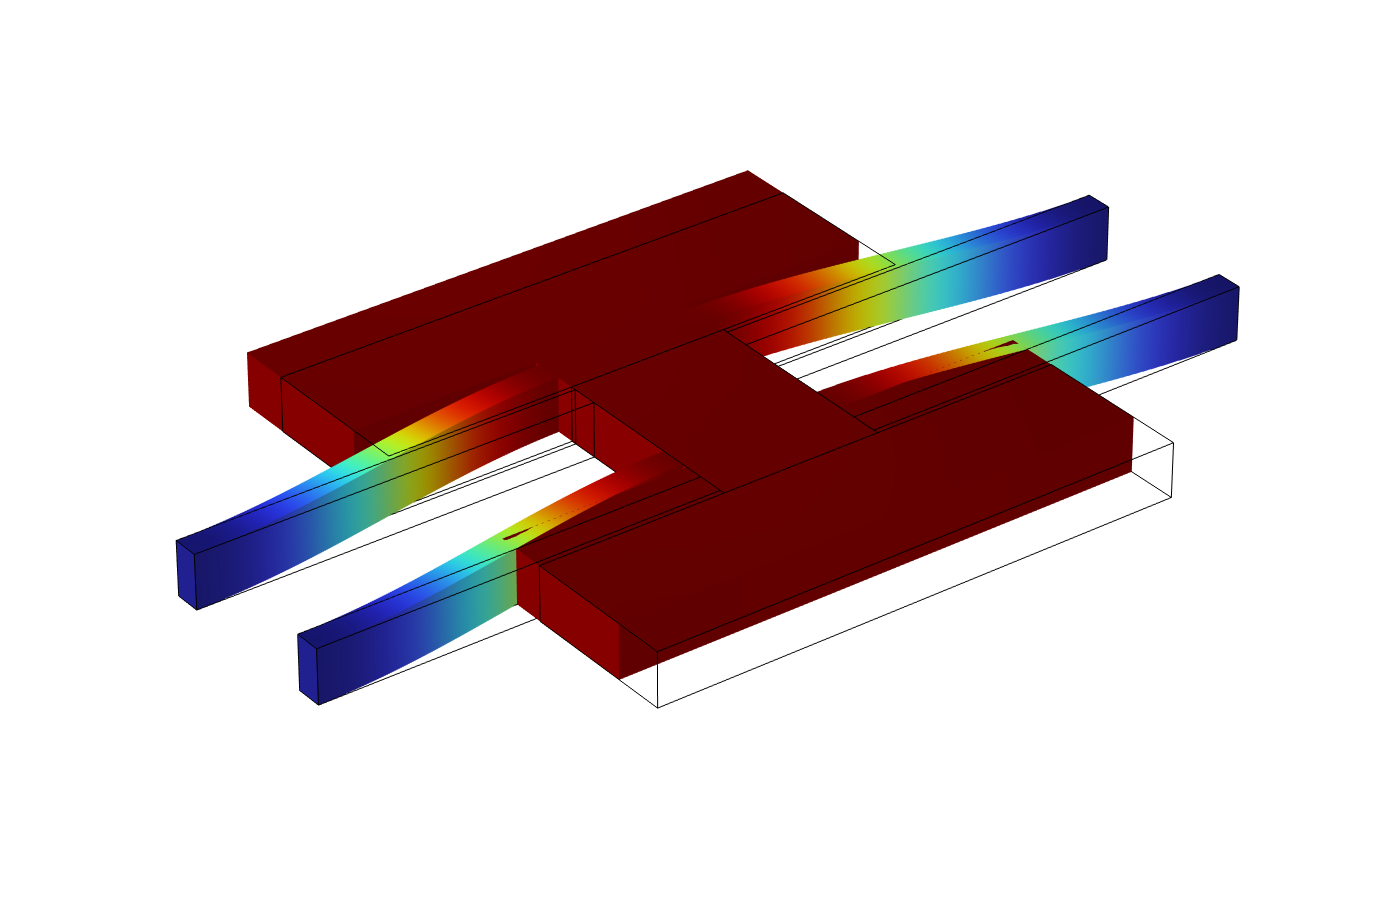
\includegraphics[width=\textwidth]{figures/p3b_mode1_515kHz.png}
  \caption{mode 1: \SI{514.8}{\kilo\hertz}, in-plane actuation}
\end{subfigure}
\begin{subfigure}{0.49\textwidth}
  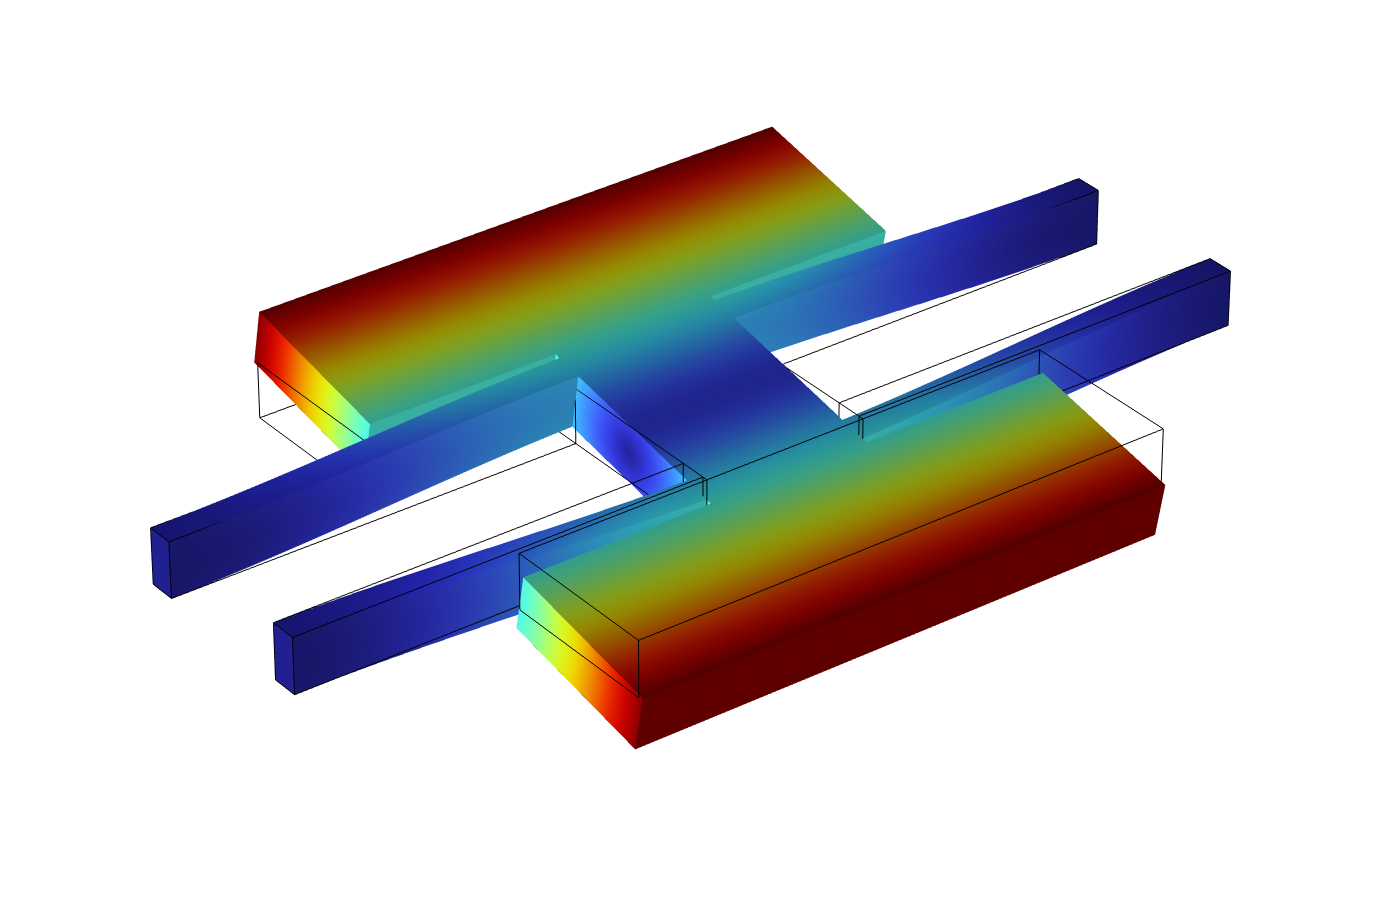
\includegraphics[width=\textwidth]{figures/p3b_mode2_608kHz.png}
  \caption{mode 2: \SI{607.9}{\kilo\hertz}, see-saw pitch}
\end{subfigure}\\[2pt]
\begin{subfigure}{0.49\textwidth}
  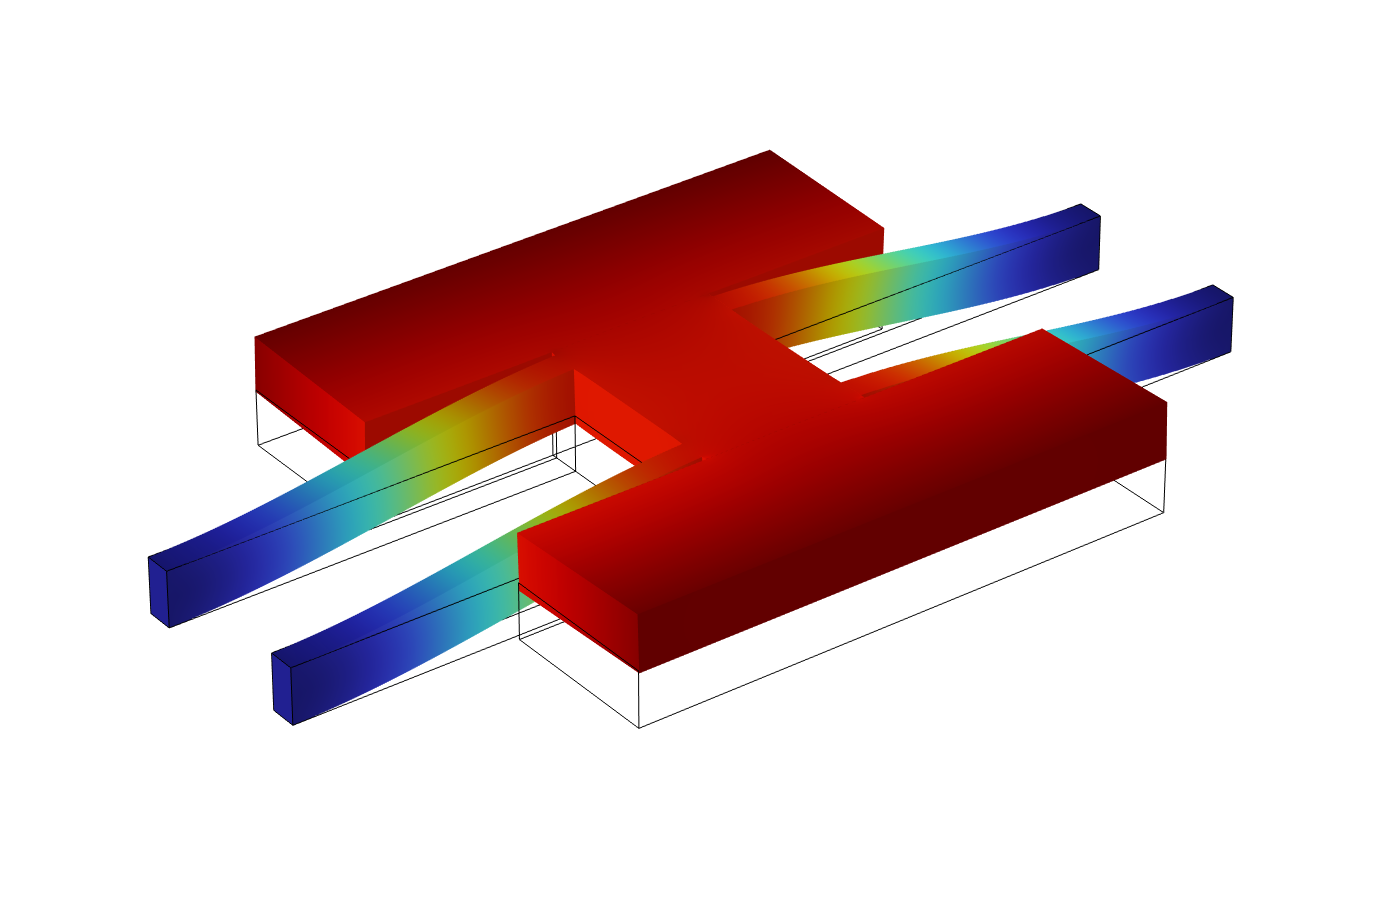
\includegraphics[width=\textwidth]{figures/p3b_mode3_928kHz.png}
  \caption{mode 3: \SI{927.9}{\kilo\hertz}, flap}
\end{subfigure}
\begin{subfigure}{0.49\textwidth}
  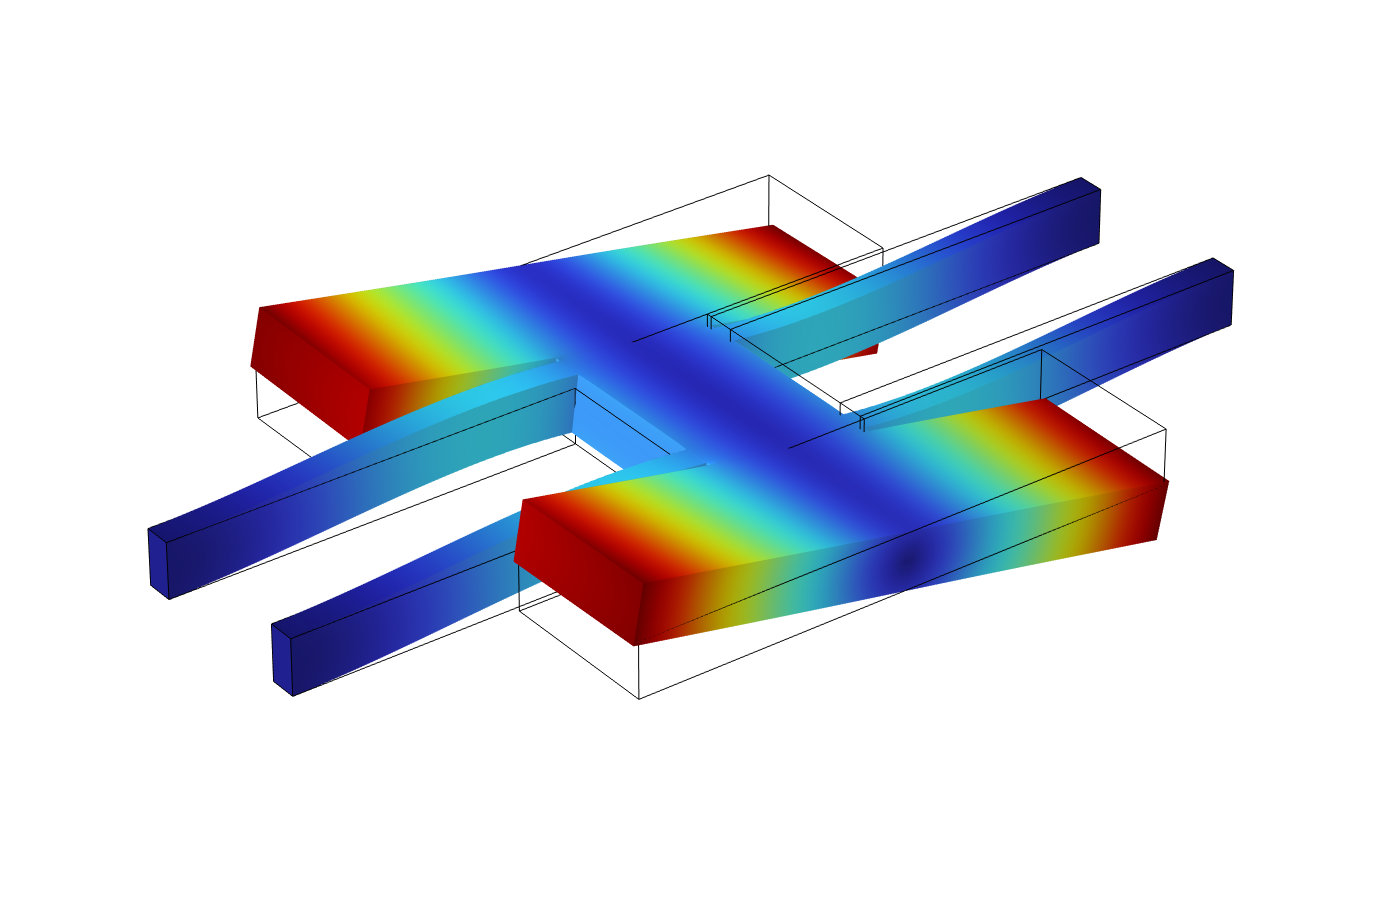
\includegraphics[width=\textwidth]{figures/p3b_mode4_1894kHz.png}
  \caption{mode 4: \SI{1894.1}{\kilo\hertz}}
\end{subfigure}\\[2pt]
\begin{subfigure}{0.6\textwidth}
  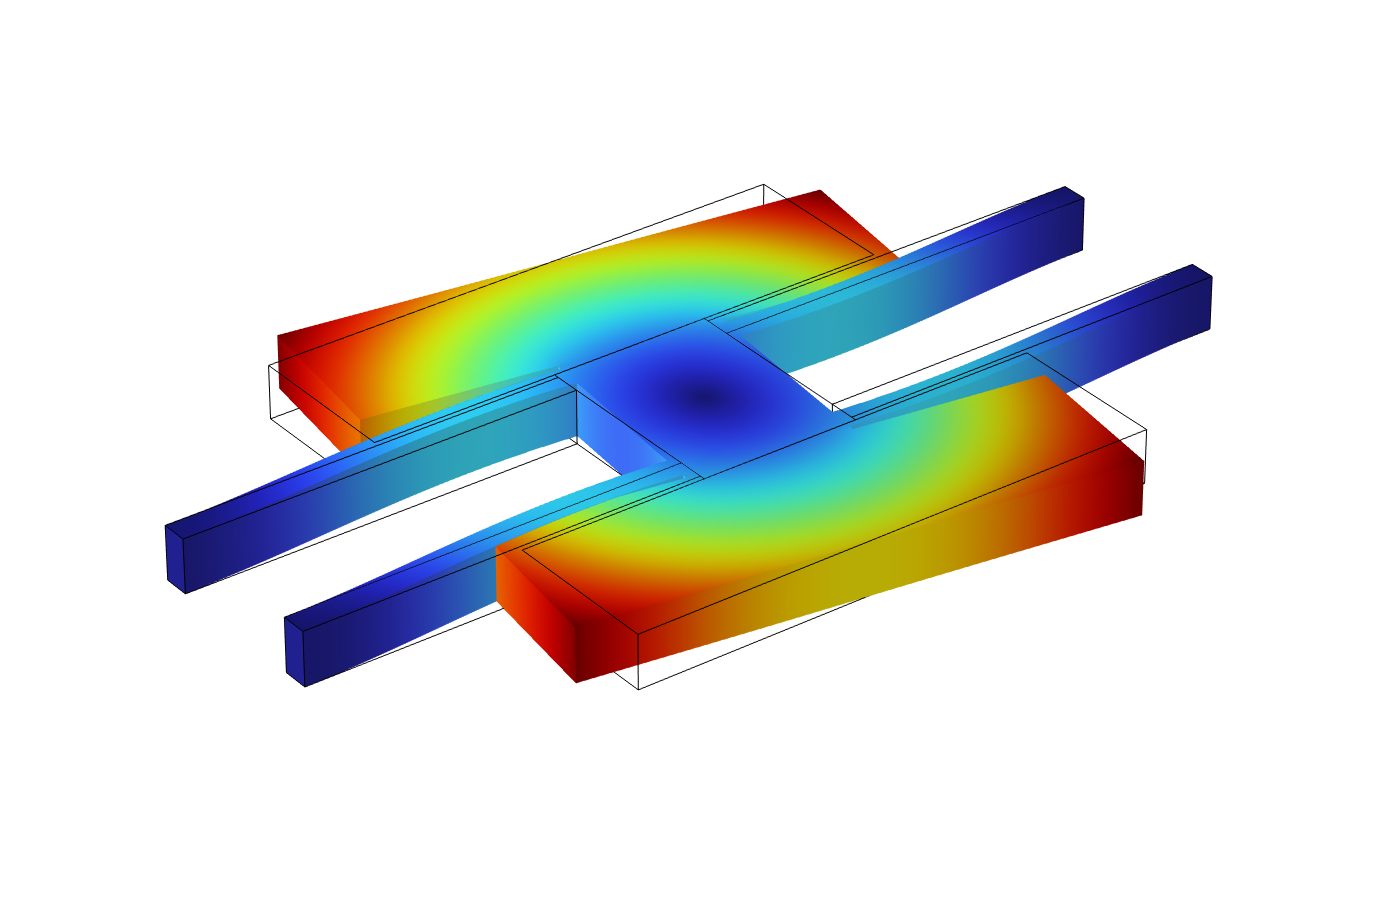
\includegraphics[width=\textwidth]{figures/p3b_mode5_2859kHz.png}
  \caption{mode 5: \SI{2858.9}{\kilo\hertz}, in-plane rotation}
\end{subfigure}
\caption{First five 3D eigenmodes at the final thickness
$t=\SI{10}{\micro\meter}$ (Part-2 dimensions, comb fingers removed).}
\label{fig:p3bmodes}
\end{figure}
